\documentclass[a4paper]{article}
\usepackage{graphicx} %Required for diagrams
\usepackage[bookmarks=true]{hyperref}
\usepackage{bookmark}%Required to do pdf bookmarking
\usepackage{booktabs}
\usepackage[margin=1.2in]{geometry}
\usepackage{float}
\usepackage{caption}
\usepackage{hyperref}%Required for referencing website pages
\usepackage[english]{babel}

\usepackage{graphicx}
\usepackage{dcolumn}
\usepackage[table]{xcolor}

\title{Burn Down And Velocity Char}
\author{Baobab Team}

\begin{document}
\newpage

\begin{titlepage}

\begin{center}


\includegraphics[width=400px]{pictures/logo.jpg}
\vspace{0.5 cm}
\begin{flushright} \large
\begin{tabular}{lr}
\vspace{1 cm}
\LARGE\textbf{Document:}Sprint Report 6\\

\vspace{1 cm}
\LARGE\textbf{Project:} Group Chat For Linphone (Agile DO-178)\\
\vspace{1 cm}
\LARGE\textbf{Advisor:} Kobus Coetzee\\
\vspace{1 cm}
\LARGE\textbf{Sponsors:} Nanoteq \& Department of Computer Science, UP\\
\vspace{1 cm}
\LARGE\textbf{Date: }\today\\
\end{tabular}
\end{flushright}

\centering 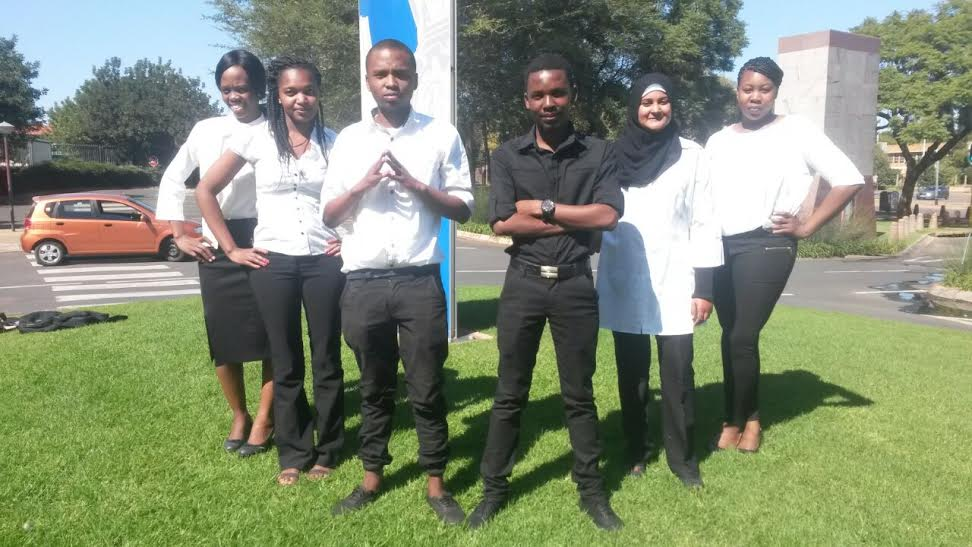
\includegraphics[width=350px]{pictures/Team.jpg}

Patience Mtsweni, Lerato Molokomme, Tsepo Ntsaba, Mpedi Mello, Lutfiyya Razak, Ephiphania Munava\\


\end{center}
\end{titlepage}
\newpage

\section{Introduction}
Scrum Product Backlog is a list of all things that we needed to implement within the project. It replaces the traditional requirements specification artifacts.

\vspace{\baselineskip}

\section{Project Details}

%Lerato edit here - System name and the names and/or affiliation of all stakeholders.
\setlength{\arrayrulewidth}{0.5mm}
\setlength{\tabcolsep}{12pt}
\renewcommand{\arraystretch}{2} 
\begin{tabular}{ |p{3cm}|p{3cm}|p{3cm}|  }
\hline
\rowcolor{lightgray}\multicolumn{2}{|c|}{System name affiliation of all stakeholders} \\
\hline
System name & Linphone Group Chat \\
\hline
Stakeholder & Kobus Coetzee \\
\hline
Scrum master  & Potego Mello\\ \hline 
Client representative  & Patience Mtsweni\\ \hline 
UX developer  & Lutfiyya Razak and Lerato Molokomme\\ \hline 
Backend developer  & Ephiphania Munava and Potego Mello\\ \hline 
Crypto developer  & Tsepo Ntsaba \\ \hline 
CI / CD support  & Patience Mtsweni \\ 
\hline
\end{tabular}
\pagebreak
 

\section{Task Description}
\begin{table} 
\begin{tabular}{p{3cm} p{1cm} p{3.5cm} p{1cm} p{1cm} p{1cm} p{1cm}} 
\hline %\toprule % Top horizontal line
& \multicolumn{5}{c}{Task Description} \\
\cmidrule(l){2-7}
Story Name & Task Number & Task Description & Status & Estimated Effort (in Hours) & Actual Effort (in Hours) & Effort Remaining (in Hours)\\ % Column names row
\hline

 & 1 & Linux & Done & 1 & 5 & 0\\ \cmidrule(l){2-6}

 & 2 & Eclipse & Done & 0.2 & 0.2 & 0\\ \cmidrule(l){2-6}

 & 3 & Android SDK & Done & 0.2  & 0.2 & 0\\ \cmidrule(l){2-6}
 
 Environment Setup & 4 & Android NDK & Done & 0.2 & 0.1 & 0\\ \cmidrule(l){2-6}

 & 5 & Android eclipse ADT & Done & 0.2 & 0.1 & 0\\ \cmidrule(l){2-6}

 & 6 & C Compiler & Done & 0.2 & 0.1 & 0\\ \cmidrule(l){2-6}
 
 & 7 & Clone Linphone project recursive & Done & 1 & 38 & 0\\ \cmidrule(l){2-6}

 & 8 &  Compile project  & Done & 2 & 48 & 0\\  
\midrule % In-table horizontal line

 Setup CI Travis & 9 & YAML File & Done & 10 & 26 & 0\\ \cmidrule(l){2-6}

 & 10 & Python File & Done & 48 & 23 & 0\\  
\midrule % In-table horizontal line

Setup CD & 11 & Devices Deployment & Done & 12 & 0.1 & 0\\
\midrule

Group Chat Interface & 12 & Activity for Each Screen & Done & 60 & 83 & 0\\ \cmidrule(l){2-6}

& 13 & Group Chat functionality Icons & Done & 20 & 15 & 0\\ 
\hline
\end{tabular}
\caption{Task Description 1} % Table caption, can be commented out if no caption is required
\label{tab:template} % A label for referencing this table elsewhere, references are used in text as \ref{label}
\end{table}

\pagebreak
 

\begin{table} 
\begin{tabular}{p{3cm} p{1cm} p{3.5cm} p{1cm} p{1cm} p{1cm} p{1cm}} 
\hline %\toprule % Top horizontal line
& \multicolumn{5}{c}{Task Description} \\
\cmidrule(l){2-7}
Story Name & Task Number & Task Description & Status & Estimated Effort (in Hours) & Actual Effort (in Hours) & Effort Remaining (in Hours)\\ % Column names row
\hline

Select Participants & 14 & List Member User-names & Done & 5 & 8 & 0\\ \cmidrule(l){2-6}

 & 15 & List Member SIP Addresses & Done & 5 & 8 & 0\\ 
\midrule

& 16 & About Button & Done & 2 & 0.5 & 0\\ \cmidrule(l){2-6}

Welcome Screen & 17 & Help Button & Done & 2 & 0.5 & 0\\ \cmidrule(l){2-6}

& 18 & Logo & Done & 0.5 & 2 & 0\\ 
\midrule

 & 19 & Group name & Done & 2 & 2 & 0\\\cmidrule(l){2-6}

Select Group Details &  20  & Group icon & Done & 2 & 2 & 0\\\cmidrule(l){2-6}

 & 21 & Exit group icon & Done & 2 & 2 & 0\\\cmidrule(l){2-6}

 & 22 & Add participants & Done & 2 & 4 & 0\\ 
 \midrule

Type Message & 23 & Type Message & Done & 1 & 2.5 & 0\\ 
 \midrule
 
 Send Message & 24 & Send Message & Done Bugs & 1 & 2.5 & 1\\ 
 \midrule
 
 Receive Message & 25 & Receive Message & Done & 1 & 2.5 & 0\\ 
 \midrule
 
 Send Picture & 26 & Send Message & Done & 4 & 2 & 0\\ 
 \midrule
 
 Receive Picture & 27 & Receive Message & Done & 4 & 3 & 0\\ 
 \midrule
 
 Record Voice & 28 & Record Voice & Done & 10 & 2 & 0\\ 
 \midrule
 
 Send Record Voice & 29 & Send Record Voice & In progress & 5 & 0 & 5\\ 
 \midrule
 
 Receive Record Voice & 30 & Receive Record Voice & In progress & 5 & 0 & 5\\ 
\hline
\end{tabular}
\caption{Task Description 2} % Table caption, can be commented out if no caption is required
\label{tab:template} % A label for referencing this table elsewhere, references are used in text as \ref{label}
\end{table}

\pagebreak


\begin{table} 
\begin{tabular}{p{3cm} p{1cm} p{3.5cm} p{1cm} p{1cm} p{1cm} p{1cm}} 
\hline %\toprule % Top horizontal line
& \multicolumn{5}{c}{Task Description} \\
\cmidrule(l){2-7}
Story Name & Task Number & Task Description & Status & Estimated Effort (in Hours) & Actual Effort (in Hours) & Effort Remaining (in Hours)\\ % Column names row
\hline

  Send Encrypted Group Messages & 31 & Send Encrypted Group Messages & Done & 38 & 68 & 18\\ 
 \midrule
 
 Receive Encrypted Group Messages & 32 & Receive Encrypted Group Messages & In progress & 20 & 27 & 10\\ 
 \midrule

 
  Send Encrypted Pictures & 33 & Send Encrypted Group Messages & In progress & 22 & 34 & 4\\ 
 \midrule
 
 Receive Encrypted Pictures & 34 & Receive Encrypted Group Messages & In progress & 10 & 14 & 5\\ 
 \midrule
 
  
  Send Encrypted Record Voice & 35 & Send Encrypted Group Messages & In progress & 22 & 34 & 4\\ 
 \midrule
 
 Receive Encrypted Record Voice & 36 & Receive Encrypted Group Messages & In progress & 10 & 14 & 5\\ 
\hline
Total Tasks & 36 & & Total & 328.9 & 473.3 & 46\\
\hline
\end{tabular}
\caption{Task Description 3} % Table caption, can be commented out if no caption is required
\label{tab:template} % A label for referencing this table elsewhere, references are used in text as \ref{label}
\end{table}

\newpage
\section{Burn Down Chat}

\pagebreak
\section{Velocity Chart}

\end{document}

